\section{Models}
\label{sec:models}

The sensor uses the photoelectric effect to produce output currents according to the following flow diagram:
\begin{figure}[H]
    \centering
    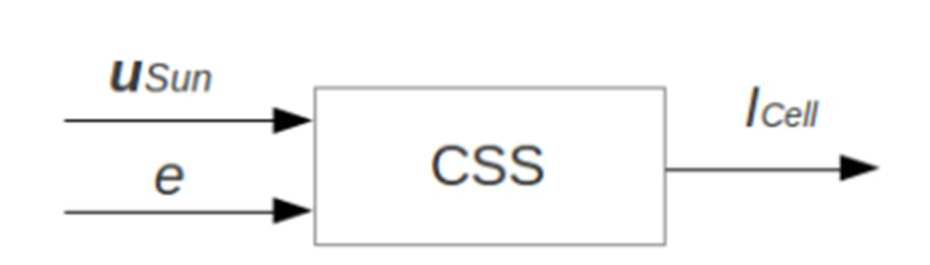
\includegraphics[width=0.5\linewidth]{doc//Graphics/sun_sensor_flowchart.png}
    \caption{Flow diagram for CSS}
    \label{fig:sun_sensor_model}
\end{figure}

The input Sun direction is given in the S/C frame. 
The CSS is also given the eclipse status of the 
S/C as a boolean $e$.
We need to take into account two configuration parameters: 1) the mounting orientation of the CSS with regard to the S/C and 2) the presence of a baffle, necessary to shield the sensor from stray light. 

\begin{figure}[H]
    \centering
    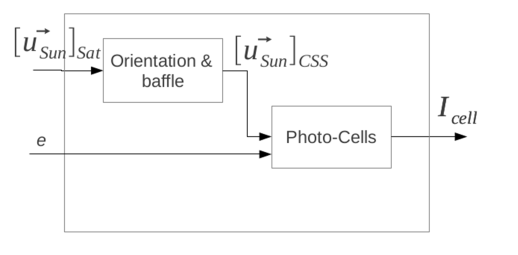
\includegraphics[width=0.75\linewidth]{Graphics/photo_cells_flowchart.png}
    \caption{Inner flow diagram for CSS}
    \label{fig:sun_sensor_inner_model}
\end{figure}

We decided to separate the model into the following submodels: \textit{Orientation and Baffle} and \textit{Cell}.
The Cell is implemented once for a single physical photo-cell and then combined in the CSS model with a total of four Cell models to accurately model the CSS.
Each submodel will be described further in the corresponding subsections below.

The configuration of the final CSS model can be seen below in \autoref{fig:CSS_model}.

\begin{figure}[H]
    \centering
    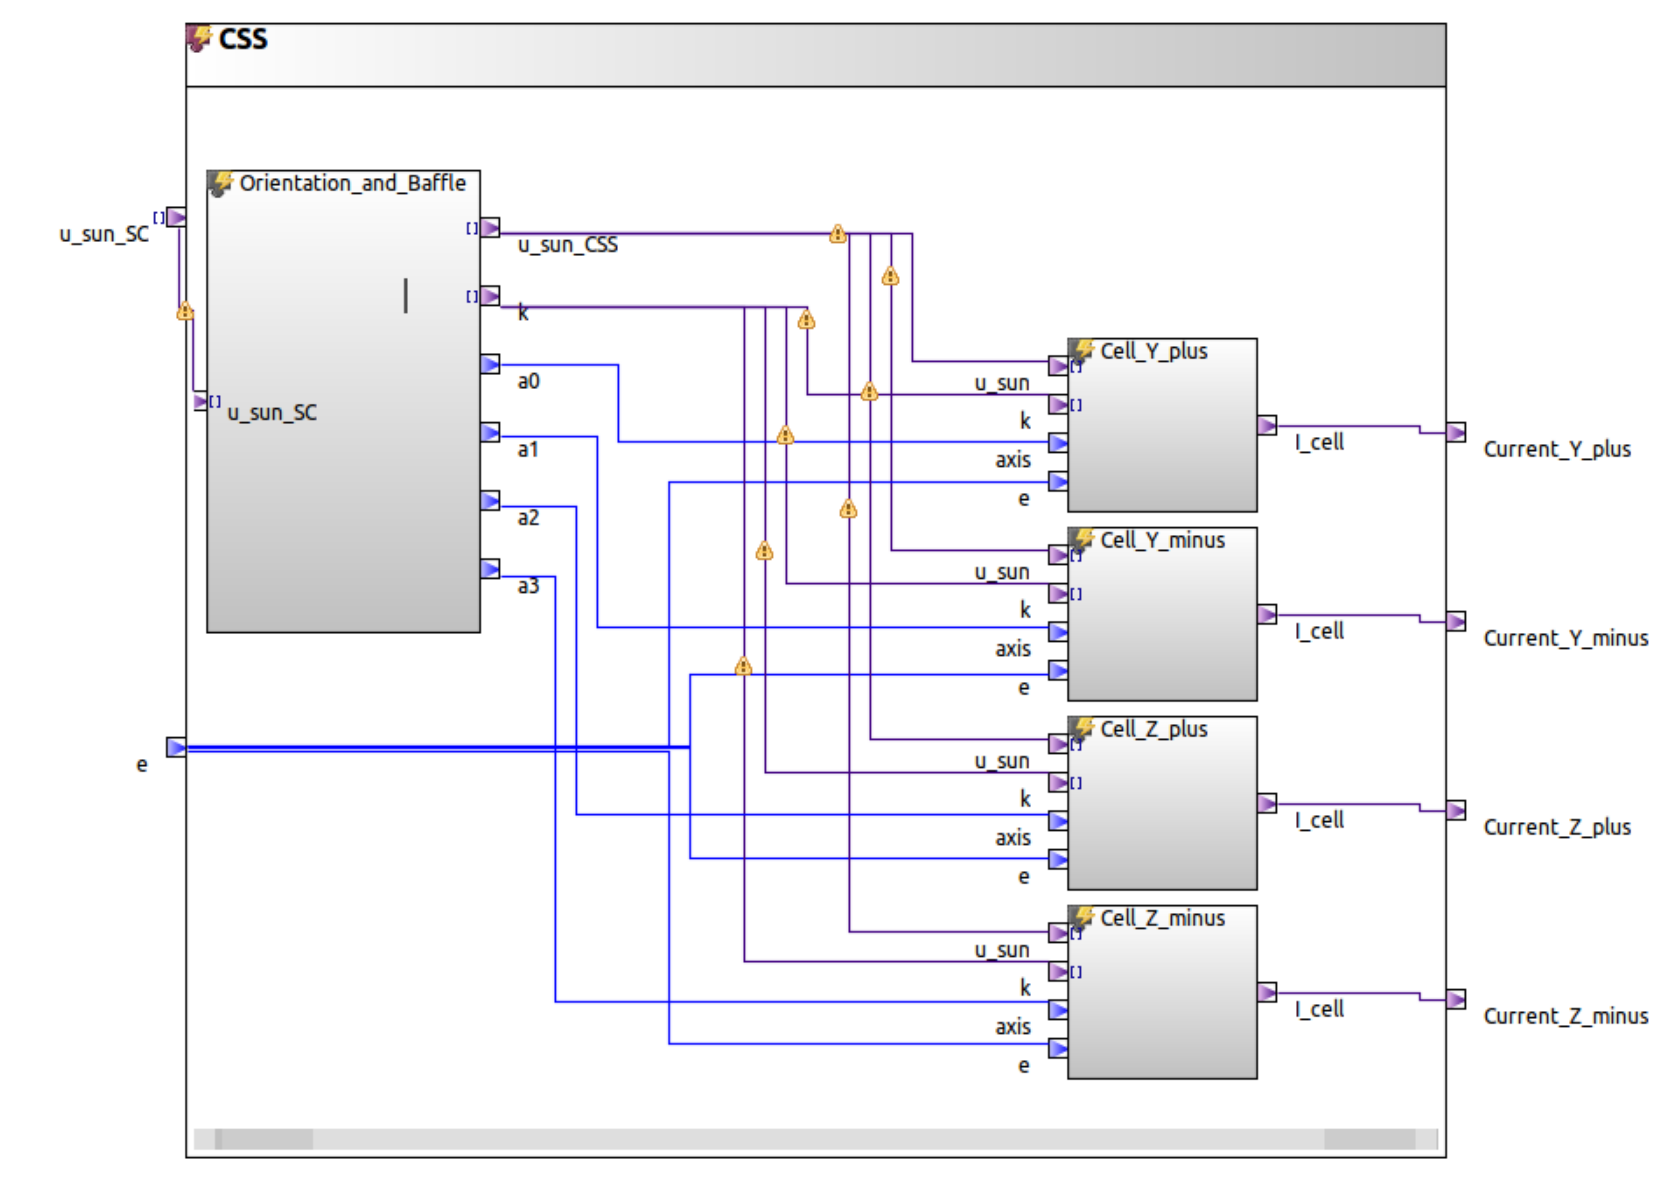
\includegraphics[width=1\linewidth]{doc//Graphics/CSS_model.png}
    \caption{SimTG model of CSS, \texttt{CSS.smf}}
    \label{fig:CSS_model}
\end{figure}

\TODO{Henkka lisää tekstiä control hommelista + see hieno lohkokaavio!}


\subsection{Single Photo-Cell}

The output current from a single photo-cell does not have a linear response curve, especially when the incident light is away from the normal to the cell. 
The output current can be modelled with the following equation:
\begin{equation}
    \begin{split}
        &I_{cell} = I_{max} \times (\Vec{n} \cdot \Vec{u_{sun}} \times \lambda \times k \times e) + N(t) \\
        &\lambda = 1 - \left( \frac{2}{\pi} \times arccos(\Vec{n} \cdot \Vec{u_{sun}})\right)^v
    \end{split}
\end{equation}
where:
\begin{itemize}
    \item $I_{max}=31 \cdot 10^{-3} \, A$ is the maximal current the cell delivers for a Sun at the cell zenith
    \item $\Vec{n}$ is a unit vector normal to the cell
    \item $\Vec{u_{sun}}$ is the sun vector which contains the x-, y-, and z- values for the sun position given to the cell as input.
    \item $v = 9.6$ is the largest incident coefficient modelling the non-linearity of the cell
    \item $k \in [0,1]$ shows the influence of the baffle on the field-of-view limitation for each cell. $k=1$ when there is no obstacle between the Sun and the cell and $k=0$ when the Sun is completely hidden from the cell.
    \item $e$ is the eclipse status (0 if satellite is in Earth shadow). 
    \item $N(t)$ is a random white noise that will be added to the output. It is bound to the constant $N_{CSS} = 2.3 \cdot 10^{-10}\, A$ and its value varies randomly.
\end{itemize}

To model the single cell, we will need as inputs the sun vector ($\Vec{u_{sun}}$), the baffle coefficient ($k$) and the eclipse status ($e$).
It will also need as input which axis it is on since the full sun sensor consists of four solar cells. 
The solar cell then uses the axis value to deduce which normal vector ($\Vec{n}$) component it shall use for the calculations.
Note that the input $k$ is an array with 4 values, which is received from the \textit{Orientation and Baffle} model such that the indexes correspond to each specific cell (+Y, -Y, +Z and -Z).
In the model the correct k-value is then selected on based on which axis the specific cell is mounted on.

The cell produces the output of $I_{cell}$ based on these inputs, according to the SimTG model the \texttt{Cell.smf}-file which is shown below in \autoref{fig:cell_model}.

\begin{figure}[H]
    \centering
    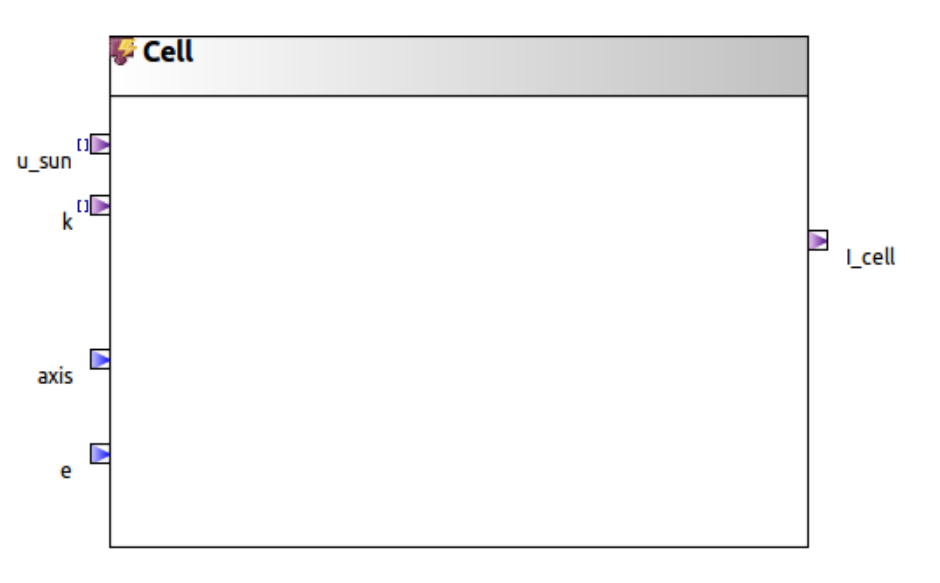
\includegraphics[width=0.75\linewidth]{doc//Graphics/cell_model.png}
    \caption{SimTG model of single photo cell, \texttt{Cell.smf}.}
    \label{fig:cell_model}
\end{figure}

\newpage
The calculation of the output current for a single photo-cell is done in a \texttt{Cell.cpp} cell, where the most relevant section is the \texttt{Cell::step()} method, which can be seen below:
\begin{lstlisting}[frame=single,
numbers=left, basicstyle=\tiny, language = C++]
void Cell::step() throw (simtg::Exception) {
	/*PROTECTED REGION ID(_bDafA9NTEe-HHfwhf86eRQ) ENABLED START*/
	float alpha = 22 * (M_PI / 180);		// sunsensor angle, converted to rad
	float I_max = 31 / 1000;			// max current in [A]
	float v = 9.6;						// largest incident coeff [-]
	float N_CSS = 2.3 * pow(10, -10)	// Noise coefficient
	float N = static_cast<float>(rand())
			/ (static_cast<float>(RAND_MAX / N_CSS)); // Noise

	float n[4][3];
	n[0] = {sin(alpha), cos(alpha), 0};		// +Y
	n[1] = {sin(alpha), -cos(alpha), 0};	// -Y
	n[2] = {sin(alpha), 0, cos(alpha)};		// +Z
	n[3] = {sin(alpha), 0, -cos(alpha)};	// -Z

	float dotProd = (_u_sun[0] * n[_axis][0]) + (_u_sun[1] * n[_axis][1])
			+ (_u_sun[2] * n[_axis][2]);

	float lambda = 1 - pow(((2 / M_PI) * acos(dotProd)), v);

	_I_cell = ((I_max * (dotProd * lambda * _k[_axis] * _e)) + N);
	/*PROTECTED REGION END*/
}
\end{lstlisting}
















\subsection{Orientation and Baffle}

The sun sensor is nominally mounted in such a way that $X_C$ is along the $-Z_S$-axis, $Y_C$ is along the $+Y_S$-axis and $Z_C$ is along the $+X_S$-axis. 
We must therefore use a rotation matrix to go from the S/C frame to the sun-sensor frame.
The used rotation matrix is:

\begin{equation}
M_R = 
\begin{bmatrix}
    cos(90^\circ) & 0 & sin(90^\circ)\\
    0 & 1 & 0 \\
    -sin(90^\circ) & 0 & cos(90^\circ)
\end{bmatrix}	
\end{equation}







\subsection{Controller}






